
%% bare_conf.tex
%% V1.4b
%% 2015/08/26
%% by Michael Shell
%% See:
%% http://www.michaelshell.org/
%% for current contact information.
%%
%% This is a skeleton file demonstrating the use of IEEEtran.cls
%% (requires IEEEtran.cls version 1.8b or later) with an IEEE
%% conference paper.
%%
%% Support sites:
%% http://www.michaelshell.org/tex/ieeetran/
%% http://www.ctan.org/pkg/ieeetran
%% and
%% http://www.ieee.org/

%%*************************************************************************
%% Legal Notice:
%% This code is offered as-is without any warranty either expressed or
%% implied; without even the implied warranty of MERCHANTABILITY or
%% FITNESS FOR A PARTICULAR PURPOSE! 
%% User assumes all risk.
%% In no event shall the IEEE or any contributor to this code be liable for
%% any damages or losses, including, but not limited to, incidental,
%% consequential, or any other damages, resulting from the use or misuse
%% of any information contained here.
%%
%% All comments are the opinions of their respective authors and are not
%% necessarily endorsed by the IEEE.
%%
%% This work is distributed under the LaTeX Project Public License (LPPL)
%% ( http://www.latex-project.org/ ) version 1.3, and may be freely used,
%% distributed and modified. A copy of the LPPL, version 1.3, is included
%% in the base LaTeX documentation of all distributions of LaTeX released
%% 2003/12/01 or later.
%% Retain all contribution notices and credits.
%% ** Modified files should be clearly indicated as such, including  **
%% ** renaming them and changing author support contact information. **
%%*************************************************************************


% *** Authors should verify (and, if needed, correct) their LaTeX system  ***
% *** with the testflow diagnostic prior to trusting their LaTeX platform ***
% *** with production work. The IEEE's font choices and paper sizes can   ***
% *** trigger bugs that do not appear when using other class files.       ***                          ***
% The testflow support page is at:
% http://www.michaelshell.org/tex/testflow/



\documentclass[conference]{IEEEtran}
% Some Computer Society conferences also require the compsoc mode option,
% but others use the standard conference format.
%
% If IEEEtran.cls has not been installed into the LaTeX system files,
% manually specify the path to it like:
% \documentclass[conference]{../sty/IEEEtran}





% Some very useful LaTeX packages include:
% (uncomment the ones you want to load)


% *** MISC UTILITY PACKAGES ***
%
%\usepackage{ifpdf}
% Heiko Oberdiek's ifpdf.sty is very useful if you need conditional
% compilation based on whether the output is pdf or dvi.
% usage:
% \ifpdf
%   % pdf code
% \else
%   % dvi code
% \fi
% The latest version of ifpdf.sty can be obtained from:
% http://www.ctan.org/pkg/ifpdf
% Also, note that IEEEtran.cls V1.7 and later provides a builtin
% \ifCLASSINFOpdf conditional that works the same way.
% When switching from latex to pdflatex and vice-versa, the compiler may
% have to be run twice to clear warning/error messages.

\usepackage{cite}
\usepackage{amsmath,amssymb,amsfonts}
\usepackage{algorithmic}
\usepackage{algorithm}
\usepackage{graphicx}
\usepackage{textcomp}
\usepackage{tikz}
\usetikzlibrary{calc,patterns,angles,quotes,shapes,arrows}


% *** CITATION PACKAGES ***
%
%\usepackage{cite}
% cite.sty was written by Donald Arseneau
% V1.6 and later of IEEEtran pre-defines the format of the cite.sty package
% \cite{} output to follow that of the IEEE. Loading the cite package will
% result in citation numbers being automatically sorted and properly
% "compressed/ranged". e.g., [1], [9], [2], [7], [5], [6] without using
% cite.sty will become [1], [2], [5]--[7], [9] using cite.sty. cite.sty's
% \cite will automatically add leading space, if needed. Use cite.sty's
% noadjust option (cite.sty V3.8 and later) if you want to turn this off
% such as if a citation ever needs to be enclosed in parenthesis.
% cite.sty is already installed on most LaTeX systems. Be sure and use
% version 5.0 (2009-03-20) and later if using hyperref.sty.
% The latest version can be obtained at:
% http://www.ctan.org/pkg/cite
% The documentation is contained in the cite.sty file itself.






% *** GRAPHICS RELATED PACKAGES ***
%
\ifCLASSINFOpdf
  % \usepackage[pdftex]{graphicx}
  % declare the path(s) where your graphic files are
  % \graphicspath{{../pdf/}{../jpeg/}}
  % and their extensions so you won't have to specify these with
  % every instance of \includegraphics
  % \DeclareGraphicsExtensions{.pdf,.jpeg,.png}
\else
  % or other class option (dvipsone, dvipdf, if not using dvips). graphicx
  % will default to the driver specified in the system graphics.cfg if no
  % driver is specified.
  % \usepackage[dvips]{graphicx}
  % declare the path(s) where your graphic files are
  % \graphicspath{{../eps/}}
  % and their extensions so you won't have to specify these with
  % every instance of \includegraphics
  % \DeclareGraphicsExtensions{.eps}
\fi
% graphicx was written by David Carlisle and Sebastian Rahtz. It is
% required if you want graphics, photos, etc. graphicx.sty is already
% installed on most LaTeX systems. The latest version and documentation
% can be obtained at: 
% http://www.ctan.org/pkg/graphicx
% Another good source of documentation is "Using Imported Graphics in
% LaTeX2e" by Keith Reckdahl which can be found at:
% http://www.ctan.org/pkg/epslatex
%
% latex, and pdflatex in dvi mode, support graphics in encapsulated
% postscript (.eps) format. pdflatex in pdf mode supports graphics
% in .pdf, .jpeg, .png and .mps (metapost) formats. Users should ensure
% that all non-photo figures use a vector format (.eps, .pdf, .mps) and
% not a bitmapped formats (.jpeg, .png). The IEEE frowns on bitmapped formats
% which can result in "jaggedy"/blurry rendering of lines and letters as
% well as large increases in file sizes.
%
% You can find documentation about the pdfTeX application at:
% http://www.tug.org/applications/pdftex





% *** MATH PACKAGES ***
%
%\usepackage{amsmath}
% A popular package from the American Mathematical Society that provides
% many useful and powerful commands for dealing with mathematics.
%
% Note that the amsmath package sets \interdisplaylinepenalty to 10000
% thus preventing page breaks from occurring within multiline equations. Use:
%\interdisplaylinepenalty=2500
% after loading amsmath to restore such page breaks as IEEEtran.cls normally
% does. amsmath.sty is already installed on most LaTeX systems. The latest
% version and documentation can be obtained at:
% http://www.ctan.org/pkg/amsmath





% *** SPECIALIZED LIST PACKAGES ***
%
%\usepackage{algorithmic}
% algorithmic.sty was written by Peter Williams and Rogerio Brito.
% This package provides an algorithmic environment fo describing algorithms.
% You can use the algorithmic environment in-text or within a figure
% environment to provide for a floating algorithm. Do NOT use the algorithm
% floating environment provided by algorithm.sty (by the same authors) or
% algorithm2e.sty (by Christophe Fiorio) as the IEEE does not use dedicated
% algorithm float types and packages that provide these will not provide
% correct IEEE style captions. The latest version and documentation of
% algorithmic.sty can be obtained at:
% http://www.ctan.org/pkg/algorithms
% Also of interest may be the (relatively newer and more customizable)
% algorithmicx.sty package by Szasz Janos:
% http://www.ctan.org/pkg/algorithmicx




% *** ALIGNMENT PACKAGES ***
%
%\usepackage{array}
% Frank Mittelbach's and David Carlisle's array.sty patches and improves
% the standard LaTeX2e array and tabular environments to provide better
% appearance and additional user controls. As the default LaTeX2e table
% generation code is lacking to the point of almost being broken with
% respect to the quality of the end results, all users are strongly
% advised to use an enhanced (at the very least that provided by array.sty)
% set of table tools. array.sty is already installed on most systems. The
% latest version and documentation can be obtained at:
% http://www.ctan.org/pkg/array


% IEEEtran contains the IEEEeqnarray family of commands that can be used to
% generate multiline equations as well as matrices, tables, etc., of high
% quality.




% *** SUBFIGURE PACKAGES ***
%\ifCLASSOPTIONcompsoc
%  \usepackage[caption=false,font=normalsize,labelfont=sf,textfont=sf]{subfig}
%\else
%  \usepackage[caption=false,font=footnotesize]{subfig}
%\fi
% subfig.sty, written by Steven Douglas Cochran, is the modern replacement
% for subfigure.sty, the latter of which is no longer maintained and is
% incompatible with some LaTeX packages including fixltx2e. However,
% subfig.sty requires and automatically loads Axel Sommerfeldt's caption.sty
% which will override IEEEtran.cls' handling of captions and this will result
% in non-IEEE style figure/table captions. To prevent this problem, be sure
% and invoke subfig.sty's "caption=false" package option (available since
% subfig.sty version 1.3, 2005/06/28) as this is will preserve IEEEtran.cls
% handling of captions.
% Note that the Computer Society format requires a larger sans serif font
% than the serif footnote size font used in traditional IEEE formatting
% and thus the need to invoke different subfig.sty package options depending
% on whether compsoc mode has been enabled.
%
% The latest version and documentation of subfig.sty can be obtained at:
% http://www.ctan.org/pkg/subfig




% *** FLOAT PACKAGES ***
%
%\usepackage{fixltx2e}
% fixltx2e, the successor to the earlier fix2col.sty, was written by
% Frank Mittelbach and David Carlisle. This package corrects a few problems
% in the LaTeX2e kernel, the most notable of which is that in current
% LaTeX2e releases, the ordering of single and double column floats is not
% guaranteed to be preserved. Thus, an unpatched LaTeX2e can allow a
% single column figure to be placed prior to an earlier double column
% figure.
% Be aware that LaTeX2e kernels dated 2015 and later have fixltx2e.sty's
% corrections already built into the system in which case a warning will
% be issued if an attempt is made to load fixltx2e.sty as it is no longer
% needed.
% The latest version and documentation can be found at:
% http://www.ctan.org/pkg/fixltx2e


%\usepackage{stfloats}
% stfloats.sty was written by Sigitas Tolusis. This package gives LaTeX2e
% the ability to do double column floats at the bottom of the page as well
% as the top. (e.g., "\begin{figure*}[!b]" is not normally possible in
% LaTeX2e). It also provides a command:
%\fnbelowfloat
% to enable the placement of footnotes below bottom floats (the standard
% LaTeX2e kernel puts them above bottom floats). This is an invasive package
% which rewrites many portions of the LaTeX2e float routines. It may not work
% with other packages that modify the LaTeX2e float routines. The latest
% version and documentation can be obtained at:
% http://www.ctan.org/pkg/stfloats
% Do not use the stfloats baselinefloat ability as the IEEE does not allow
% \baselineskip to stretch. Authors submitting work to the IEEE should note
% that the IEEE rarely uses double column equations and that authors should try
% to avoid such use. Do not be tempted to use the cuted.sty or midfloat.sty
% packages (also by Sigitas Tolusis) as the IEEE does not format its papers in
% such ways.
% Do not attempt to use stfloats with fixltx2e as they are incompatible.
% Instead, use Morten Hogholm'a dblfloatfix which combines the features
% of both fixltx2e and stfloats:
%
% \usepackage{dblfloatfix}
% The latest version can be found at:
% http://www.ctan.org/pkg/dblfloatfix




% *** PDF, URL AND HYPERLINK PACKAGES ***
%
%\usepackage{url}
% url.sty was written by Donald Arseneau. It provides better support for
% handling and breaking URLs. url.sty is already installed on most LaTeX
% systems. The latest version and documentation can be obtained at:
% http://www.ctan.org/pkg/url
% Basically, \url{my_url_here}.




% *** Do not adjust lengths that control margins, column widths, etc. ***
% *** Do not use packages that alter fonts (such as pslatex).         ***
% There should be no need to do such things with IEEEtran.cls V1.6 and later.
% (Unless specifically asked to do so by the journal or conference you plan
% to submit to, of course. )


% correct bad hyphenation here
\hyphenation{op-tical net-works semi-conduc-tor}


\begin{document}
%
% paper title
% Titles are generally capitalized except for words such as a, an, and, as,
% at, but, by, for, in, nor, of, on, or, the, to and up, which are usually
% not capitalized unless they are the first or last word of the title.
% Linebreaks \\ can be used within to get better formatting as desired.
% Do not put math or special symbols in the title.
%\title{Bare Demo of IEEEtran.cls\\ for IEEE Conferences}
\tableofcontents
\title{ROCO504\\ Catch-bot}

% author names and affiliations
% use a multiple column layout for up to three different
% affiliations
\author{\IEEEauthorblockN{Tom Queen}
\IEEEauthorblockA{School of Computing,\\ Electronics and Mathematics\\
Plymouth University\\
Plymouth, Devon PL4 8AA \\
Email: xxxx}
\and
\IEEEauthorblockN{Daniel Gregory-Turner}
\IEEEauthorblockA{School of Computing,\\ Electronics and Mathematics\\
	Plymouth University\\
	Plymouth, Devon PL4 8AA \\
	Email: xxxx}
\and
\IEEEauthorblockN{Demetrius Zaibo}
\IEEEauthorblockA{School of Computing,\\ Electronics and Mathematics\\
	Plymouth University\\
	Plymouth, Devon PL4 8AA \\
	Email: xxxx}}

% conference papers do not typically use \thanks and this command
% is locked out in conference mode. If really needed, such as for
% the acknowledgment of grants, issue a \IEEEoverridecommandlockouts
% after \documentclass

% for over three affiliations, or if they all won't fit within the width
% of the page, use this alternative format:
% 
%\author{\IEEEauthorblockN{Michael Shell\IEEEauthorrefmark{1},
%Homer Simpson\IEEEauthorrefmark{2},
%James Kirk\IEEEauthorrefmark{3}, 
%Montgomery Scott\IEEEauthorrefmark{3} and
%Eldon Tyrell\IEEEauthorrefmark{4}}
%\IEEEauthorblockA{\IEEEauthorrefmark{1}School of Electrical and Computer Engineering\\
%Georgia Institute of Technology,
%Atlanta, Georgia 30332--0250\\ Email: see http://www.michaelshell.org/contact.html}
%\IEEEauthorblockA{\IEEEauthorrefmark{2}Twentieth Century Fox, Springfield, USA\\
%Email: homer@thesimpsons.com}
%\IEEEauthorblockA{\IEEEauthorrefmark{3}Starfleet Academy, San Francisco, California 96678-2391\\
%Telephone: (800) 555--1212, Fax: (888) 555--1212}
%\IEEEauthorblockA{\IEEEauthorrefmark{4}Tyrell Inc., 123 Replicant Street, Los Angeles, California 90210--4321}}




% use for special paper notices
%\IEEEspecialpapernotice{(Invited Paper)}




% make the title area
\maketitle

% As a general rule, do not put math, special symbols or citations
% in the abstract
\begin{abstract}
The abstract goes here.
\end{abstract}

% no keywords




% For peer review papers, you can put extra information on the cover
% page as needed:
% \ifCLASSOPTIONpeerreview
% \begin{center} \bfseries EDICS Category: 3-BBND \end{center}
% \fi
%
% For peerreview papers, this IEEEtran command inserts a page break and
% creates the second title. It will be ignored for other modes.
\IEEEpeerreviewmaketitle



\section{Introduction}
% no \IEEEPARstart
This demo file is intended to serve as a ``starter file''
for IEEE conference papers produced under \LaTeX\ using
IEEEtran.cls version 1.8b and later.
% You must have at least 2 lines in the paragraph with the drop letter
% (should never be an issue)
I wish you the best of success.

\hfill mds
 
\hfill August 26, 2015

\subsection{Subsection Heading Here}
Subsection text here.


\subsubsection{Subsubsection Heading Here}
Subsubsection text here.


% An example of a floating figure using the graphicx package.
% Note that \label must occur AFTER (or within) \caption.
% For figures, \caption should occur after the \includegraphics.
% Note that IEEEtran v1.7 and later has special internal code that
% is designed to preserve the operation of \label within \caption
% even when the captionsoff option is in effect. However, because
% of issues like this, it may be the safest practice to put all your
% \label just after \caption rather than within \caption{}.
%
% Reminder: the "draftcls" or "draftclsnofoot", not "draft", class
% option should be used if it is desired that the figures are to be
% displayed while in draft mode.
%
%\begin{figure}[!t]
%\centering
%\includegraphics[width=2.5in]{myfigure}
% where an .eps filename suffix will be assumed under latex, 
% and a .pdf suffix will be assumed for pdflatex; or what has been declared
% via \DeclareGraphicsExtensions.
%\caption{Simulation results for the network.}
%\label{fig_sim}
%\end{figure}

% Note that the IEEE typically puts floats only at the top, even when this
% results in a large percentage of a column being occupied by floats.


% An example of a double column floating figure using two subfigures.
% (The subfig.sty package must be loaded for this to work.)
% The subfigure \label commands are set within each subfloat command,
% and the \label for the overall figure must come after \caption.
% \hfil is used as a separator to get equal spacing.
% Watch out that the combined width of all the subfigures on a 
% line do not exceed the text width or a line break will occur.
%
%\begin{figure*}[!t]
%\centering
%\subfloat[Case I]{\includegraphics[width=2.5in]{box}%
%\label{fig_first_case}}
%\hfil
%\subfloat[Case II]{\includegraphics[width=2.5in]{box}%
%\label{fig_second_case}}
%\caption{Simulation results for the network.}
%\label{fig_sim}
%\end{figure*}
%
% Note that often IEEE papers with subfigures do not employ subfigure
% captions (using the optional argument to \subfloat[]), but instead will
% reference/describe all of them (a), (b), etc., within the main caption.
% Be aware that for subfig.sty to generate the (a), (b), etc., subfigure
% labels, the optional argument to \subfloat must be present. If a
% subcaption is not desired, just leave its contents blank,
% e.g., \subfloat[].


% An example of a floating table. Note that, for IEEE style tables, the
% \caption command should come BEFORE the table and, given that table
% captions serve much like titles, are usually capitalized except for words
% such as a, an, and, as, at, but, by, for, in, nor, of, on, or, the, to
% and up, which are usually not capitalized unless they are the first or
% last word of the caption. Table text will default to \footnotesize as
% the IEEE normally uses this smaller font for tables.
% The \label must come after \caption as always.
%
%\begin{table}[!t]
%% increase table row spacing, adjust to taste
%\renewcommand{\arraystretch}{1.3}
% if using array.sty, it might be a good idea to tweak the value of
% \extrarowheight as needed to properly center the text within the cells
%\caption{An Example of a Table}
%\label{table_example}
%\centering
%% Some packages, such as MDW tools, offer better commands for making tables
%% than the plain LaTeX2e tabular which is used here.
%\begin{tabular}{|c||c|}
%\hline
%One & Two\\
%\hline
%Three & Four\\
%\hline
%\end{tabular}
%\end{table}


% Note that the IEEE does not put floats in the very first column
% - or typically anywhere on the first page for that matter. Also,
% in-text middle ("here") positioning is typically not used, but it
% is allowed and encouraged for Computer Society conferences (but
% not Computer Society journals). Most IEEE journals/conferences use
% top floats exclusively. 
% Note that, LaTeX2e, unlike IEEE journals/conferences, places
% footnotes above bottom floats. This can be corrected via the
% \fnbelowfloat command of the stfloats package.


\section{Design Process}
\subsection{Problem}
\subsubsection{Inverse Kinematics}\label{initial_kinematics}
Initially it was thought that the commands to each motor could be generated by looking directly at the returned X and Y coordinates of the tracked objects. To move the gripper upwards, the top two motors should rotate clockwise and the bottom two anticlockwise. To move the gripper to the left, the two left motors should rotate clockwise and the right two anticlockwise. This led to the following kinematic solution:
\begin{equation}
\begin{aligned}
&M1 = Y - X \\
&M2 = Y + X\\
&M3 = -Y -X\\
&M4 = -Y + X\\
\end{aligned}
\end{equation}
For high torque motors, elastic cords and a closed loop between the tracked object and the gripper, this approximation would have been functional. However, it would not have been accurate and it would unnesicarrily load the motors. When using stepper motors with low-current drivers, this solution caused the steppers to skip if the gripper was directed more than a few centimeters from the centre of the working area. 
This led to re-evaluation of the kinematic solution as can be seen in section \ref{kinematic_solution_1}.

\subsubsection{Force storage} \label{force_problem}


\subsubsection{Camera speed}
In order to track the target quickly, a low latency high FPS camera was needed.
\subsubsection{Motors}
Fast motors were needed to allow the gripper to keep track of the target. The working area of the frame measured XXXX 90cm by 75cm. If the gripper was initialised to the centre of the frame and a ball was thrown from three meters away, then the robot would have 0.7 seconds to move from center to the corner of the working area. PROOF
\subsection{Research}
\subsection{Requirements}

\subsection{Solutions}
To achieve the required speed and torque, several motor solutions were designed. 
\subsubsection{Micro motors}\label{gearbox_sol}
The first was to use high torque (300Ncm) encoded DC motors (E192.24.125). The maximum speed of these motors was 33rpm. In order to achieve the required gripper speed of 1.5m/s, a gearbox was needed.
\begin{equation}
\begin{aligned}
\frac{s}{\pi\cdot d \cdot r} = \frac{150}{\pi\cdot 10 \cdot 0.55} = 1:8.68
\end{aligned}
\end{equation}
Where $d$ is the spool diameter ($10cm$), $s$ is required cord speed ($150cm/s$) and $r$ is motor speed ($0.55 \ RPM$). This ratio would result in a maximum cord velocity of $149.9 cm/s$.\\ 
\subsubsection{Stepper motors}
Another solution was to use stepper motors. Four SST58D3820 stepper motors were acquired. These motors are specified to hold $7.3Kg.cm$, which drops to $6.5Kg.cm$ at a frequency of 1200 pulses per second (PPS). The motors step size was $1.8\textdegree$, giving a max speed of 6RPS and thus a maximum cord velocity of $188.5cm/s$. \begin{equation}
\begin{aligned}
\frac{1.8\cdot 1200}{360} = 6 RPS
\end{aligned}
\end{equation}
\begin{equation}
\begin{aligned}
6\cdot\pi\cdot 10 = 188.49cm/s
\end{aligned}
\end{equation}
\subsubsection{Clamps}
To address the problem discussed in \ref{force_problem}, clamps were designed to lock each cord in place. Each clamp consisted of a high-friction surface suspended above a fixed plate via four springs. The cord to be clamped runs between the two surfaces. A dynamixel AX-12 servo is connected the suspended surface with a pulley. When actuated, the servo pulls the suspended surface towards the fixed plate, closing the gap and clamping the cord in place. A clamp was produced for each of the five cords, one for each corner of the frame and one for the throwing motor.

\subsubsection{Camera}
The Sony Playstation3 eye camera can be purchased second-hand for 50p. This camera can output 187 frames per second (FPS) at a resolution of 320x240, or 60 FPS at a resolution of 640x480. In addition, the camera allows for control of exposure, gain, white balance, saturation and hue shift.
\subsubsection{Kinematic solution 1} \label{kinematic_solution_1}
To address the issues discussed in \ref{initial_kinematics}, the following kinematic model was produced.
\begin{figure}
	\centering
	
	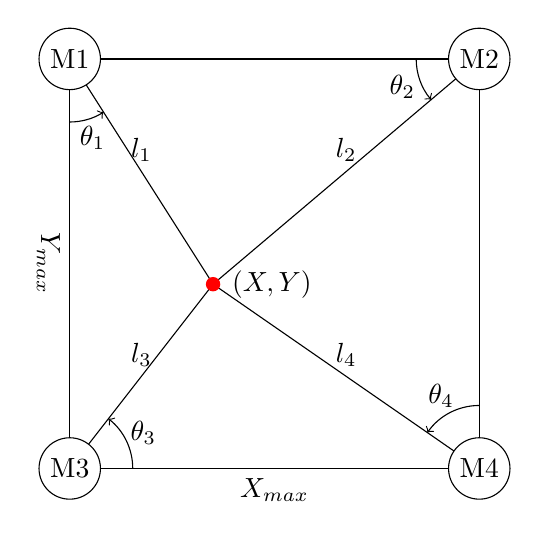
\begin{tikzpicture}[scale=1.3]
	
	\draw (0,0) -- (4,0) node[midway,below] {$X_{max}$} -- (4,4) -- (0,4) -- cycle node[midway,below,sloped] {$Y_{max}$}  ;
	
	\coordinate (M1) at (0,4);
	\coordinate (M2) at (4,4);
	\coordinate (M3) at (0,0);
	\coordinate (M4) at (4,0);
	\coordinate[label=right:{$\ (X,Y)$}] (c) at (1.4, 1.8);
	\draw (c) -- (0,0) node[midway,above] {$l_3$} ;
	\draw (c) -- (0,4) node[midway,above] {$l_1$} ;
	\draw (c) -- (4,0) node[midway,above] {$l_4$} ;
	\draw (c) -- (4,4) node[midway,above] {$l_2$} ;
	%\draw ()
	\fill[red] (c) circle (2pt);
	
	
	\draw[fill=white] (M3) circle (0.3cm) node[text=black] {M3};
	
	\draw[fill=white] (M1) circle (0.3cm) node[text=black] {M1};
	
	\draw[fill=white] (M4) circle (0.3cm) node[text=black] {M4};
	
	\draw[fill=white] (M2) circle (0.3cm) node[text=black] {M2};
	
	\pic [draw, angle radius=0.8cm, ->, "$\theta_1$", angle eccentricity=1.3] {angle = M3--M1--c};
	
	\pic [draw, angle radius=0.8cm, ->, "$\theta_2$", angle eccentricity=1.3] {angle = M1--M2--c};
	
	\pic [draw, angle radius=0.8cm, ->, "$\theta_4$", angle eccentricity=1.3] {angle = M2--M4--c};
	
	\pic [draw, angle radius=0.8cm, ->, "$\theta_3$", angle eccentricity=1.3] {angle = M4--M3--c};
	
	\end{tikzpicture}
	\caption{Kinematic diagram} \label{fig:K_diag_1}
\end{figure}

Inverse Kinematics:
\begin{equation}
\cos(\theta_3) = \frac{X_{max}{}^2 + l_3{}^2 - l_4{}^2}{2*X_{max}*l_3}
\end{equation}
\begin{equation}
X = l_3\sin(\theta_3)
\end{equation}
\begin{equation}
Y = l_3\cos(\theta_3)
\end{equation}

Or, without trigonometry:

\begin{equation} \label{inverse_kinematics_1}
\begin{aligned}
&X = \left(\frac{X_{max}{}^2 + l_3{}^2 - l_4{}^2}{2*X_{max}*l_3}\right) = \frac{X_{max}}{2} + \frac{l_3{}^2 - l_4{}^2}{2*X_{max}}\\ \\
&Y = \left(\frac{Y_{max}{}^2 + l_4{}^2 - l_1{}^2}{2*Y_{max}*l_3}\right) = \frac{Y_{max}}{2} + \frac{l_4{}^2 - l_1{}^2}{2*Y_{max}}
\end{aligned}
\end{equation}

Forward Kinematics:
\begin{equation} \label{forward_kinematics_1}
\begin{aligned}
&l_1 = \sqrt{\left(X\right)^2 + \left(Y_{max}-Y\right)^2}\\
&l_2 = \sqrt{\left(X_{max}-X\right)^2 + \left(Y_{max}-Y\right)^2}\\
&l_3 = \sqrt{\left(X\right)^2 + \left(Y\right)^2}\\
&l_4 = \sqrt{\left(X_{max}-X\right)^2 + \left(Y\right)^2}\\
\end{aligned}
\end{equation}
\subsection{Prototype}
\subsubsection{Hardware}
These solutions led to the development of the initial prototype. This robot used four stepper motors to drive the gripper. Each motor was driven by a HST-8325B stepper driver with control signals generated on a teensy3.2 running the arduino firmware. 
\subsubsection{Software}
The teensy was using the rosserial library to receive the targets CofM from the computer. The teensy then offset the coordinate system so that pixel 0,0 was in the centre of the image. The teensy kept track of all motor positions, and when a new CofM arrived the current gripper position was calculated from the motor positions using the forward kinematics described by equation \ref{forward_kinematics_1} in \ref{kinematic_solution_1}. The program generates motor commands designed to move the gripper so that the centre of the camera image contains the CofM of the target. This is known as visual servoing. The x and y error between the centre of the camera image and the target is calculated, generating a vector that points towards the target. This vector is translated into the change in length of each cord required to center the gripper over the tracked target using the inverse kinematics described by equation \ref{inverse_kinematics_1} in \ref{kinematic_solution_1}. The desired gripper location is checked to see if it has left the bounds of the working area. If it has, movement in the direction of the axis which has been breached is set to zero. Finally, motor speeds are calculated from the desired changes in lengths as is described in equation \ref{motor_speed_equation} in section \ref{motor_speed_section}.
\subsection{Further problems}
\subsubsection{Gearbox}
A gearbox ratio of 1:8.68 was chosen as can be seen in \ref{gearbox_sol}. If a 500g gripper were to be raised along either vertical wall of the workspace, the output of the gearbox raising it would experience $5Kg.cm$ of force. Transferring this force through the gearbox, a 1cm input gear would experience $43.4 Kg.cm$ of force. By making the length of each gear inversely proportional to its accumulated speed multiplier, the stress felt by the input gear could be spread out over the rest of the gears. However, as this would have more than doubled the size of our original gearbox (SIZESXXXXXXXXXXX), the decision was made to use stepper motors instead.
\subsubsection{Stepper Drivers}
Four HST-8325B were purchased to drive the SST58D3820 stepper motors. The HST-8325B is designed to deliver up to 3.5A RMS. The drivers current can be limited down to 0.8A RMS in eight steps. The performance in the SST58D3820 datasheet is rated for when the motors are being supplied with 2.0A per phase. From this we can see that the stepper motor requires 250mA per phase more than the driver can provide. 
An issue arose 

drivers were connected to the stepper motors and the current to the driver was measured, the stepper driver 
\subsubsection{Skipping steps}\label{motor_issues}
The prototype was assembled with SST58D3820 stepper motors and HST-8325B drivers. When the robot was switched on the motors could barely hold the weight of the gripper when stationary. An experiment was performed where commands were sent to the robot instructing the gripper to move to the top corner and then return to the centre with cord lengths measured before and after. It was found that requesting any movement of the gripper resulted in the stepper motors skipping steps, often resulting in the gripper dropping tens of centimetres over short movements. Further investigation showed that the stepper drivers were drawing minimal current, and would overheat and shutdown if their current limit was set to more than half of what they were rated for. Even with a current limit set at 2.0A RMS, each stepper never drew more than 1.0A. This issue could have been partly mitigated if the motors were encoded.
\subsubsection{Kinematics} \label{kinematic_solution_3}
Initially the kinematic solution considered the gripper as a point. This worked for preliminary testing, but soon proved to be a problem when the limited torque of the stepper motors required equal tension on all cords at all times. This led to the development of the following kinematic model, which considered the gripper as a square. 

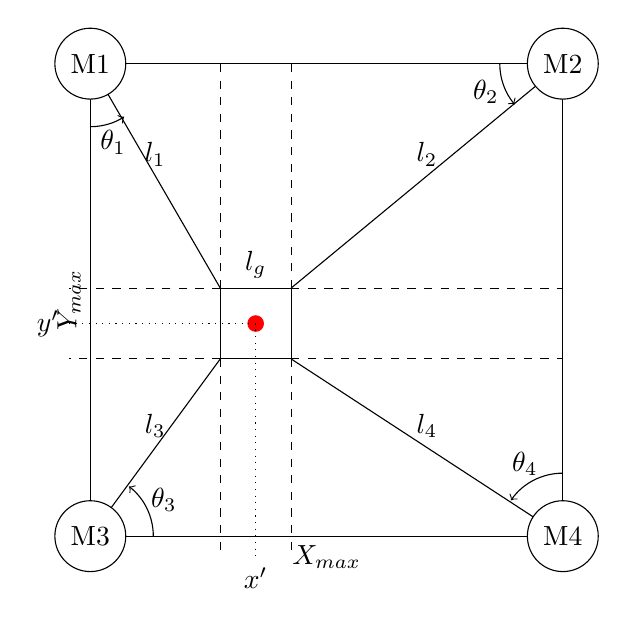
\begin{tikzpicture}[scale=1.5]

\def\gripSize{0.3}
%\pgfmathsetmacro{\grip_size}{0.3}

\coordinate (M1) at (0,4);
\coordinate (M2) at (4,4);
\coordinate (M3) at (0,0);
\coordinate (M4) at (4,0);

\draw (M3)--(M4) node[midway,below] (xaxis) {$X_{max}$};
\draw (M4)--(M2) node[midway,above](yaxisr){};
\draw (M1)--(M2) node[midway,right](xaxist){};
\draw (M3)--(M1) node[midway,above,sloped] (yaxis) {$Y_{max}$}  ;

%\draw (M3,M1) node (yaxis){};

\coordinate (c) at (1.4, 1.8);
\coordinate (c1) at ($(c) + (-\gripSize,\gripSize)$);
\coordinate (c2) at ($(c) + (\gripSize,\gripSize)$);
\coordinate (c3) at ($(c) + (-\gripSize,-\gripSize)$);
\coordinate (c4) at ($(c) + (\gripSize,-\gripSize)$);
\draw (c1) -- (0,4) node[midway,above] {$l_1$} ;
\draw (c2) -- (4,4) node[midway,above] {$l_2$} ;
\draw (c3) -- (0,0) node[midway,above] {$l_3$} ;
\draw (c4) -- (4,0) node[midway,above] {$l_4$} ;

%\draw ()
\fill[red] (c) circle (2pt);

\draw[dotted] (yaxis |- c) node[left] {$y'$}
-| (xaxis -| c) node[below] {$x'$};

\draw[dashed] (c3) -- (xaxis -| c3) ;
\draw[dashed] (c3) -- (yaxis |- c3) ;

\draw[dashed] (c1) -- (xaxist -| c1) ;
\draw[dashed] (c1) -- (yaxis |- c1) ;

\draw[dashed] (c2) -- (xaxist -| c2) ;
\draw[dashed] (c2) -- (yaxisr |- c2) ;
\draw[dashed] (c4) -- (xaxis -| c4) ;
\draw[dashed] (c4) -- (yaxisr |- c4) ;

\draw (c1) -- (c2) node[midway,above] {$l_g$} -- (c4) -- (c3) -- cycle;

\draw[fill=white] (M1) circle (0.3cm) node[text=black] {M1};

\draw[fill=white] (M2) circle (0.3cm) node[text=black] {M2};

\draw[fill=white] (M3) circle (0.3cm) node[text=black] {M3};

\draw[fill=white] (M4) circle (0.3cm) node[text=black] {M4};



\pic [draw, angle radius=0.8cm, ->, "$\theta_1$", angle eccentricity=1.3] {angle = M3--M1--c};

\pic [draw, angle radius=0.8cm, ->, "$\theta_2$", angle eccentricity=1.3] {angle = M1--M2--c};

\pic [draw, angle radius=0.8cm, ->, "$\theta_4$", angle eccentricity=1.3] {angle = M2--M4--c};

\pic [draw, angle radius=0.8cm, ->, "$\theta_3$", angle eccentricity=1.3] {angle = M4--M3--c};

\end{tikzpicture}
\linebreak

Inverse Kinematics:

\begin{equation}
\begin{aligned}
&X = \frac{X_{max}}{2} + \frac{l_3{}^2 - l_4{}^2}{2\left(X_{max} - l_g\right)}\\ \\
&Y = \frac{Y_{max}}{2} + \frac{l_3{}^2 - l_4{}^2}{2\left(Y_{max} - l_g\right)}\\
\end{aligned}
\end{equation}

Forward Kinematics:

\begin{equation}
\begin{aligned}
&l_1 = \sqrt{\left(X - \frac{l_g}{2}\right)^2 + \left(Y_{max}-Y+\frac{l_g}{2}\right)^2}\\
&l_2 = \sqrt{\left(X_{max}-X+\frac{l_g}{2}\right)^2 + \left(Y_{max}-Y+\frac{l_g}{2}\right)^2}\\
&l_3 = \sqrt{\left(X-\frac{l_g}{2}\right)^2 + \left(Y-\frac{l_g}{2}\right)^2}\\
&l_4 = \sqrt{\left(X_{max}-X+\frac{l_g}{2}\right)^2 + \left(Y-\frac{l_g}{2}\right)^2}\\
\end{aligned}
\end{equation}
\subsubsection{Motor velocities}\label{motor_vel_problem}
For the tension to remain equal on all cords during motion of the gripper, the motors must turn at different rates. For example: if the gripper starts in the centre of the frame and moves upwards, the top two lengths will shorten and the bottom two cords will get longer. To maintain a uniform velocity of the gripper, the top two motors must slow down and the bottom two must speed up.
\subsubsection{Motors}
\subsubsection{Arduino}
\subsection{Redesign}
\subsubsection{Motor velocities}\label{motor_speed_section}
To address the issue raised in \ref{motor_vel_problem} a simple speed scaling system was devised. This algorithm was called once per main loop after the required changes in lengths are calculated. The algorithm takes in the requested changes in length of each cord and divides each change in length by the largest. The algorithm then scales the relative speeds of each motor by the global speed scalar.
\begin{equation}\label{motor_speed_equation}
\begin{aligned}
&\vec{l} = \begin{bmatrix}
l_1\\l_2\\l_3\\l_4\\
\end{bmatrix}\quad
%&x = \max\{l_1,...,l_4\}\\
&x = \max\{l\}\\\\
&\vec{s} = \frac{g}{x}\cdot \vec{l}\\
%&s_1 = \frac{l_1}{x}\\
%&s_2 = \frac{l_2}{x}\\
%&s_3 = \frac{l_3}{x}\\
%&s_4 = \frac{l_4}{x}\\
\end{aligned}
\end{equation}
Where $g$ is the global speed scalar and $s$ contains the speed of each motor.
\subsubsection{Servos}
Due to the points mentioned in \ref{motor_issues}, the decision was made to change the motors to Dynamixel MX-64 servos. The MX-64 can supply $0.6Kg.cm$ at 62 RPM, giving a top gripper speed of $0.32m/s$ which is considerably slower than our requirement. The MX-64 servos communicate over either a RS-485 or a TTL bus and can be daisy-chained if required. 
\subsection{Final solution}


\section{Implementation}
\subsection{Software}
Frames enter the object tracking node at a rate of 60FPS. The object tracker performs a series of filters in different colour spaces on the image before calculating its centre of mass. This coordinate is published to the kinematic controller 17.5ms after the frame enters the object tracker. Upon entering the kinematic controller, the coordinate frame is offset so that the center of the camera image is now at pixel 0,0. The required change in length of each cord is then calculated and set (via the method described in \ref{kinematic_solution_3}). From the desired changes in length, the required speed of each motor is calculated and set. The kinematic controller node then calculates the current gripper position in order to calculate the changes in length for the next loop.
Figure~\ref{fig:HighLevelDiagram} shows the high-level software flow diagram of the robot.
\begin{figure}[htbp]
	\centerline{%
		\resizebox{0.3\textwidth}{!}{\includegraphics{ROCO504-overall.png}}%
	}
	\caption{High-level software flow diagram.}
	\label{fig:HighLevelDiagram}
	\end{figure}
	

	% Define block styles
	\tikzstyle{decision} = [diamond, draw, fill=blue!20, 
	text width=4.5em, text badly centered, node distance=3cm, inner sep=0pt]
	
	\tikzstyle{block} = [rectangle, draw, 
	text width=5em, text centered, rounded corners, minimum height=4em]
	
	\tikzstyle{square} = [rectangle, draw, 
	text width=5em, text centered, minimum height=4em, minimum width=7em]
	
	\tikzstyle{sectionb} = [rectangle, draw, dotted, minimum height=18em, minimum width=20em, distance=0cm]
	
	\tikzstyle{sectiona} = [rectangle, draw, dotted, minimum height=15em, minimum width=20em, distance=0cm]
	
	\tikzstyle{line} = [draw, -latex']
	\tikzstyle{cloud} = [draw, ellipse,fill=red!20, node distance=3cm,
	minimum height=2em]
	
	\begin{tikzpicture}[node distance = 2cm,transform shape, scale=0.8]
	% Place nodes
	\node [square] (filter) {Filtering};
	\node [block, left of=filter, node distance=3cm] (camera) {camera};
	\node [square, below of=filter] (CofM) {Centre of Mass};
	\node [square, below of=CofM, node distance=3cm] (lengthCal) {Calculate/set new lengths};
	\node [square, below of=lengthCal] (speedCal) {Calculate/set speeds};
	\node [block, left of=speedCal, node distance=3cm] (motors) {Motors};
	\node [square, below of=speedCal] (gripperPos) {Find gripper position};
	\node [sectionb, left of=speedCal, node distance =1cm] (section1) {};
	\node [sectiona, below left of=filter, node distance =1cm] (section1) {};
	\node [right of = gripperPos] (dir1){};
	\node [above of = dir1] (dir2){};
		\node [above of = dir2] (dir3){};
	% Draw edges
	\path [line] (camera) -- (filter);
	\path [line] (filter) -- (CofM);
	\path [line] (CofM) -- (lengthCal);
	%\path [line] (lengthCal) -- (gripperPos);
	\path [line] (lengthCal) -- (speedCal);
	\path [line] (speedCal) -- (gripperPos);
	\path [line] (lengthCal) -- (motors);
	\path [line] (speedCal) -- (motors);
	\path [line] (motors) -- (gripperPos);
	\draw [-] (gripperPos) -- (dir1);
	\draw [->] (dir1) -- (dir2);
		\draw [->] (dir2) -- (dir3);
		\draw [->] (dir3) -- (lengthCal);
	%\path [line] (decide) -| node [near start] {yes} (update);
	%\path [line] (update) |- (identify);
	%\path [line] (decide) -- node {no}(stop);
	%\path [line,dashed] (expert) -- (init);
	%\path [line,dashed] (system) -- (init);
	%\path [line,dashed] (system) |- (evaluate);
	\end{tikzpicture}
	
\subsection{Frame}
\subsection{Kinematics}
\subsection{Grippers}
\subsection{Clamps}

\section{Experiments}
\subsection{Method}
\subsection{Results}
\subsection{Discussion}
\section{Overall Discussion}


\section{Conclusion}
The conclusion goes here.




% conference papers do not normally have an appendix


% use section* for acknowledgment
\section*{Acknowledgment}


The authors would like to thank...





% trigger a \newpage just before the given reference
% number - used to balance the columns on the last page
% adjust value as needed - may need to be readjusted if
% the document is modified later
%\IEEEtriggeratref{8}
% The "triggered" command can be changed if desired:
%\IEEEtriggercmd{\enlargethispage{-5in}}

% references section

% can use a liography generated by BibTeX as a .bbl file
% BibTeX documentation can be easily obtained at:
% http://mirror.ctan.org/biblio/bibtex/contrib/doc/
% The IEEEtran BibTeX style support page is at:
% http://www.michaelshell.org/tex/ieeetran/bibtex/
\bibliographystyle{IEEEtran}
% argument is your BibTeX string definitions and bibliography database(s)
%\bibliography{IEEEabrv,../bib/paper}
%
% <OR> manually copy in the resultant .bbl file
% set second argument of \begin to the number of references
% (used to reserve space for the reference number labels box)
\begin{thebibliography}{1}
	

				\bibitem{Simpson} Homer J. Simpson. \textsl{Mmmmm...donuts}.
				Evergreen Terrace Printing Co., Springfield, SomewhereUSA, 1998

				\bibitem{rosserial} ROSserial Wiki \textsl{Mmmmm...donuts}.
				Evergreen Terrace Printing Co., Springfield, SomewhereUSA, 1998
				

					
@online{rosserial,
	author = {Misc},
	title = {Rosserial wiki},
	date = {30/12/17},
	url = {http://wiki.ros.org/rosserial},
}
\bibitem{IEEEhowto:kopka}
H.~Kopka and P.~W. Daly, \emph{A Guide to \LaTeX}, 3rd~ed.\hskip 1em plus
  0.5em minus 0.4em\relax Harlow, England: Addison-Wesley, 1999.

	
\bibitem{b1} G. Eason, B. Noble, and I. N. Sneddon, ``On certain integrals of Lipschitz-Hankel type involving products of Bessel functions,'' Phil. Trans. Roy. Soc. London, vol. A247, pp. 529--551, April 1955.
\bibitem{b2} J. Clerk Maxwell, A Treatise on Electricity and Magnetism, 3rd ed., vol. 2. Oxford: Clarendon, 1892, pp.68--73.
\bibitem{b3} I. S. Jacobs and C. P. Bean, ``Fine particles, thin films and exchange anisotropy,'' in Magnetism, vol. III, G. T. Rado and H. Suhl, Eds. New York: Academic, 1963, pp. 271--350.
\bibitem{b4} K. Elissa, ``Title of paper if known,'' unpublished.
\bibitem{b5} R. Nicole, ``Title of paper with only first word capitalized,'' J. Name Stand. Abbrev., in press.
\bibitem{b6} Y. Yorozu, M. Hirano, K. Oka, and Y. Tagawa, ``Electron spectroscopy studies on magneto-optical media and plastic substrate interface,'' IEEE Transl. J. Magn. Japan, vol. 2, pp. 740--741, August 1987 [Digests 9th Annual Conf. Magnetics Japan, p. 301, 1982].
\bibitem{b7} M. Young, The Technical Writer's Handbook. Mill Valley, CA: University Science, 1989.
	
\end{thebibliography}


% that's all folks
\end{document}


